Gentry's work was a true breakthrough. It not only presented the first, fully homomorphic encryption scheme, but also gave researchers a very powerful tool, the \textit{bootstrapping}. From now on, all we need to construct another FHE scheme, is some suitable (one requirement would be to use a scheme based on ring rather than a group) SHE method, apply appropriate "squashing" to obtain the bootstrapping and we are done. In the following years this is exactly what happened in academia and the industry.

This section will mostly serve as a survey of the main developments towards more efficient fully homomorphic encryption using (ideal) lattices and their security based on computational hardness of the underlying problems. We adopt chronological narrative of the sections, starting with the oldest, the GGH algorithm, progressing through works on (ring-)LWE and eventually arriving at the work of Gentry \cite{gentry_phd} on ideal lattices and FHE. For a good survey on the lattice based cryptography, see for example \cite{two_faces}, \cite{book} chapter 6 or \cite{lattice-survey}.

\subsection{The GGH public key cryptosystem}
We will start this section with a somewhat simpler cryptosystem that was developed by Goldreich, Goldwasser and Halevi and presented in 1997 \cite{ggh}, called the GGH cryptosystem. This scheme, rather than using ideal lattices (i.e. lattices that are also ideals in the ring of integers), relies on general properties of lattices. Namely, the hardness of the SVP and CVP (see section \ref{hardness}).

\subsubsection*{Idea behind the scheme}
The basic GGH cryptosystem, as mentioned before, is based on the problem of finding the closest vector in the lattice $\mathcal{L}$ to a given point in the ambient space $\R^n$. We are given two bases, call them $\Bg$ and $\Bb$. The $\Bb$ will be our public key and $\Bg$ the secret key. The $\Bb$ consists of long and highly non-orthogonal vectors, as opposed to $\Bg$. Our secret message $\bm{m}$ is represented as a binary vector which we will use to form a linear combination $\bm{s} = \sum m_i \bm{v}_i^{bad} \in \mathcal{L}$ of the vectors in $\Bb$. We now add some small and random\footnote{some small note about the "randomness" of this e} error $\bm{e} \in \R^n$ to obtain the ciphertext $\bm{c} = \bm{s} + \bm{e} = \sum m_i \bm{v}_i^{bad} + \bm{e} \in \R^n$ - some point that is not in the lattice, but rather, very close to a point in it.\\
To decrypt, we can use our good basis $\Bg$ to represent $\bm{c}$ and, for example Babai's algorithm\footnote{Simply stated, if the vectors of the basis are sufficiently orthogonal to one another, then this algorithm solves \prob{approxCVP}. However, if the Hadamard ratio is too small, the algorithm fails to find the closest vector - \cite{book}.} to find $\bm{v}$ and represent it in terms of the basis $\Bg$ to recover $\bm{m}$. On the other hand, any eavesdropping adversary that is trying to learn our secret, is left with some bad basis that will be of no help in solving the CVP.

\subsubsection*{GGH construction - concretely}
\noindent\fbox{%
    \parbox{\textwidth}{%
$\alg{KeyGen}$:
\begin{itemize}
    \item Pick a basis $(\bm{v}_1, \bm{v}_2, \dots, \bm{v}_n) \subset \Z^n$ such that they are reasonably orthogonal to one another - i.e. with small Hadamard ratio. We will associatie the vectors $\bm{v}_1, \bm{v}_2, \dots, \bm{v}_n$ as the $n$-by-$n$ matrix $\bm{V}$ and let $\mathcal{L}$ be the lattice generated by these vectors. This is our good basis $\Bg$ - the \textbf{private key}.
    \item Pick an $n$-by-$n$ matrix $\bm{U}$ with integer coefficients and determinant $\pm 1$ and compute $\bm{W} = \bm{UV}$. The column vectors $\bm{w}_1, \bm{w}_2, \dots, \bm{w}_n$ of $\bm{W}$ are the bad basis $\Bb$ of $\mathcal{L}$ - the \textbf{public key}\footnote{As an alternative, in \cite{hnf}, Micciancio suggested to use the Hermite Normal Form (HNF) of $\Bg$ which essentially provides the worst possible lattice choice from both cryptoanalitical and efficiency point of view.}.
\end{itemize}
$\alg{Encrypt}$:
$\alg{Decrypt}$:
}} \\

The greatest drawback of GGH is that there were no proofs of security presented along the algorithm, only heuristic assumptions. This motivated researchers to look for possible exploits beased on the choice of parameters. Indeed, this scheme turned out to be insecure for most practical choices of the security parameter only 2 years later, in \cite{break1} and broken completely in \cite{break2}. Nonetheless, the ideas presented there have served as a basis for many schemes that are proven to be secure, like for example LWE, and has led to a plethora of applications.
\subsection{Learning With Errors}
Let us now begin with what went wrong in GGH. Namely, first prove the hardness of a problem, then use it to construct a secure and efficient cryptosystem. In this section we introduce \textit{Learning With Errors} (LWE) problem and the cryptosystem introduced by Oded Regev in \cite{regev} (he won the \href{https://eatcs.org/index.php/component/content/article/1-news/2670-2018-godel-prize}{2018 Gödel Prize} for this work). This very important work in the field of lattice based cryptography is, up to the date \krzys{im not sure if this statement is true, i need to look more into it}, one of the most efficient schemes with an actual proof of security. It has served as a foundation for countless subsequent works in the field. \krzys{provide validation for this statement}

\iffalse
\subsubsection*{Lattices - Part II}

\begin{definition}[Dual]
    For a lattice $\mathcal{L} \subset \R^n$ its $\Z$\textit{-dual} is
    $$ \mathcal{L}^{\vee} = \{ y \in \R^n : y \cdot \mathcal{L} \subset \Z \}.$$
    Here, the $\cdot$ means the usual dot product.
\end{definition}

We simply require that the elements of the dual are precisely those vectors that yield an integer when "multiplied" with an element of our lattice. Note that this is different from our standard definition of a dual. Namely, it is not the orthogonal compliment of our starting space, i.e. not all of the elements of the dual have 0 dot product against the vectors of the lattice.

\begin{example}
    Take $\mathcal{L}= \Z 
        \big(\begin{smallmatrix} 1\\2 \end{smallmatrix}\big) + 
        \Z \big(\begin{smallmatrix} 0\\ 1 \end{smallmatrix}\big)$
        To calculate the dual of $\mathcal{L}$ we need our $y = \big(\begin{smallmatrix}
          a\\b\end{smallmatrix}\big)$ elements to satisfy $a \in \Z$ and $2a + b \in \Z$ which is equivalent to asking $a \in (1/2)\Z$ and so $\mathcal{L}^{\vee} = \big(\begin{smallmatrix}
          1/2\\0
        \end{smallmatrix}\big)\Z + \big(\begin{smallmatrix}
          0\\1
        \end{smallmatrix}\big) \Z$
\end{example}

Note that $\mathcal{L}^{\vee}$ is itself a lattice of the same dimension.
\fi

\subsubsection*{LWE problem}
There are multiple equivalent definitions of this problem. We adopt the notation and approach introduced in the original paper by Regev. In this section, we will mainly focus on the parts that are the most relevant for our study of ring-LWE.\\

The problem is parametrized by positive integers $n$, $m$\footnote{As will be seen later, $m$ is of secondary importance here and is usually taken to be equal to $n$ itself.} and prime $q$, as well as an error distibution $\chi$ over $\Z_q$. It is now defined as follows. We are given $m$ equations of the form $(\bm{a}_i, b_i = \langle \bm{a}_i, \bm{s} \rangle + e_i)$ and are asked to find the vector $\bm{s} \in \Z_q^n$. Here, $\bm{a}_i$ are chosen uniformly and independently from $\Z_q^n$, $b_i \in \Z_q$ and $\langle \cdot, \cdot \rangle$ denotes the usual dot product. The errors $e_i$ are obtained by sampling independently from the probability distribution $\chi : \Z_q \rightarrow \R^{+}$ on $\Z_q$. We will denote the problem of recovering $\bm{s}$ from such equations, by $\text{LWE}_{q, \chi}$ (learning with errors).

\begin{example}[From the introduction to \cite{regev_survey}]\label{lwe_ex}
    Given as input this set of equations, LWE asks us to recover the vector $\bm{s} = (s_1, s_2, s_3, s_4) \in \Z_{17}^4$. In this case $n = 4$, $q=17$ and the error distribution is giving us $e_i = \{-1, 1\}$ with equal probability. 
\begin{align*}
    14s_1 + 15s_2 +5s_3 + 2s_4 & \approx 8 \, (\mod 17)\\
    13s_1 + 14s_2 + 14s_3 + 6s_4 & \approx 16\, (\mod 17) \\
    6s_1 + 10s_2 + 13s_3 + 1s_4 & \approx 3\, (\mod 17) \\
    10s_1 + 4s_2 + 12s_3 + 16s_4 & \approx 12\, (\mod 17) \\
    9s_1 + 5s_2 + 9s_3 +6s_4 & \approx 9\, (\mod 17) \\
    3s_1 + 6s_2 +4s_3 +5s_4 & \approx 16\, (\mod 17) \\
    \vdots & \\
    6s_1 + 7s_2 + 16s_3 + 2s_4 & \approx 3\, (\mod 17)
\end{align*}
In this case, $\bm{s} = (0, 13, 9, 11)$. Note that if not for the error, the secret would be very easy to find. Given about $n$ equations, we could recover $\bm{s}$ in an efficient way using Gaussian elimination. Inducing the error is what seems to render the problem untraceable for modern day algorithms.
\end{example}

The central part of \cite{regev} revolves around proving the hardness of LWE. Specifically, that for appropriately chosen $q$ and $\chi$, a \textit{quantum}\footnote{In fact, quantum reduction is used only in the small part of the whole proof.} reduction algorithm exists that approximates worst-case lattice problems. 
\begin{remark}
    At some point as well, we would like to find entirely \textit{classical} reduction algorithm that proves the hardness of the problem. This is because we understand classical computation in much more detail than its quantum equivalent. Using classical computers we have cracked Enigma and landed on the moon. In the meantime, only recently a factorization of the integer 15 was achieved on a quantum computer using Shor's algorithm - see \krzys{find source of that statement}. Returning to the reduction problem, Chris Peikert in his paper \cite{peikert_classical} from 2009 has done exactly this. However, it was done in a somewhat ``inefficient'' way. That is, exponentially many samples are needed in the classical reduction compared to polynomial amount in the quantum version. For more details see the paper by Peikert and compare it with the original approach from Regev. It remains an important open question \krzys{also not sure about that} till this day, if the reduction can be made efficiently fully classical.
\end{remark}
This result is stated as follows (with small changes).

\begin{theorem}[\cite{regev} Theorem 1.1]\label{main}
    Let $n$, $q$ be positive integers and $\alpha \in (0, 1)$ be such that $\alpha q > 2 \sqrt{n}$. If there exists an efficient algorithm that solves $\text{LWE}_{q, \bar{\Psi}_{\alpha}}$, then there exists an efficient quantum algorithm that approximates the decision version of the shortest vector problem (\prob{GapSVP}) and the shortest independent vectors problem (\prob{SIVP}) to within $\tilde{O}(n/\alpha)$ in the worst case on any lattice of dimension $n$.	
\end{theorem}

Let us unwrap this statement. As said before, we need an appropriate choice of paramenters to obtain our results and $\alpha > 2\sqrt{n}/q$ is one of those choices (and requirements). It specifies the shape of the $\bar{\Psi}_{\alpha}$ distribution. This one is almost identical to the discrete Gaussian distribution over $\Z_q$ that is centered around 0 with standard deviation $\alpha q$\footnote{A comment from \cite{lattice-survey}: Originally, Regev considered the continuous Gaussian and rounded the result to the nearest integer. This does not exactly yield the discrete distribution but thanks to \cite{discr} we know how the problem can be fixed.}. The theorem can be rephrased as follows. Imagine that we have an efficient algorithm that solves the $\text{LWE}_{q, \bar{\Psi}_{\alpha}}$. Then, there exists a quantum solution to worst-case lattice problems, namely \prob{GapSVP} and \prob{SIVP}. Since we strongly believe that \prob{GapSVP} and \prob{SIVP} are difficult to solve (\cite{svp-hard}, \cite{reductions}, \cite{cvp-hard}) we are left with a difficult, yet efficient way to share secrets. Oded Regev proceeds to prove this using various lemmas and results from few areas of mathematics like probability, lattice theory and quantum computing. We will now present an outline of the approach.

\paragraph{Proof of Theorem \ref{main}}
Recall that we want to prove, that being able to solve $\text{LWE}_{q, \chi}$ implies that we are able to solve standard worst-case lattice problems like \prob{GapSVP}. To achieve this, we need to proceed in steps, in other words, we perform reductions from one problem to another. Before we proceed any further, let us define some terminology first.

From this point on, a probabilistic algorithm which solves a given $\text{LWE}_{q, \chi}$ instance, will be called an LWE-\textit{oracle} (or, when there is no confusion, simply an oracle). Hence, let us assume that we have such an oracle that solves $\text{LWE}_{q, \chi}$. The main idea presented by Regev is the so called \textit{iterative step}. On each of the iterations, it is using the oracle to produce discrete Gaussian samples of smaller and smaller radius around our desired \textit{closest vector}. Once we have a sample with radius small enough, we can use that to output a solution to the \prob{GapSVP} and \prob{SIVP} as stated in Theorem \ref{main}.

\begin{center}
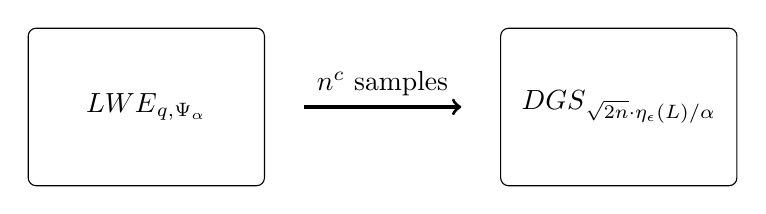
\begin{tikzpicture}
% Define the left box
\draw[rounded corners=1mm] (0,0) rectangle (3,2);
\node at (1.5,1) {$\text{LWE}_{q, \Psi_{\alpha}}$};

% Define the right box
\draw[rounded corners=1mm] (6,0) rectangle (9,2);
\node at (7.5,1) {$\text{DGS}_{\sqrt{2n} \cdot \eta_{\epsilon}(L)/\alpha}$};

% Define the arrow between the boxes
\draw[->, very thick] (3.5,1) -- node[above] {$n^c$ samples} (5.5,1);
\end{tikzpicture}
\end{center}

The algorithm can be divided into two basic steps, the classical step and the quantum step. 

\begin{center}
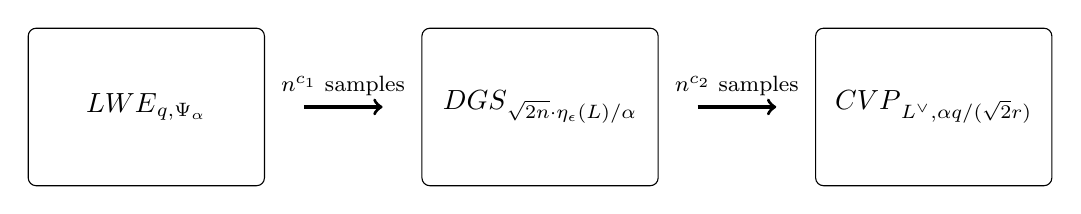
\begin{tikzpicture}
\draw[rounded corners=1mm] (0,0) rectangle (3,2);
\node at (1.5,1) {$\text{LWE}_{q, \Psi_{\alpha}}$};

\draw[->, very thick] (3.5,1) -- node[above] {\footnotesize $n^{c_1}$ samples} (4.5,1);

\draw[rounded corners=1mm] (5,0) rectangle (8,2);
\node at (6.5,1) {$\text{DGS}_{\sqrt{2n} \cdot \eta_{\epsilon}(L)/\alpha}$};

\draw[->, very thick] (8.5,1) -- node[above] {\footnotesize $n^{c_2}$ samples} (9.5,1);

\draw[rounded corners=1mm] (10,0) rectangle (13,2);
\node at (11.5, 1) {$\text{CVP}_{L^{\vee}, \alpha q / (\sqrt{2} r)}$};

\end{tikzpicture}
\end{center}
As said in the introduction, we will focus on the first (classical) step in the reduction from LWE to \prob{DGS} as it is what is altered the most in the ring-LWE hardness proof. This, however, will follow in the next section.
\paragraph{The classical step}
The following statement (Theorem 3.1 in \cite{regev}) is the core of the hardness results of LWE. For example, later it is (\krzys{or maybe i'll include as well}) proven the equivalence between search LWE and decision LWE. This is very important result as it is usually much easier to construct cryptographic schemes based on some \textit{decision} version of a problem rather than the \textit{search}.
\begin{theorem}[3.1 \cite{regev}]
    Let $q \geq 2$ be an integer and $\alpha$ be a real number in $(0, 1)$. Assume we are given access to an oracle that solves the LWE problem with modulus $q$ and error parameter $\alpha$. Then, given as input any lattice $\Lambda$, a large enough polynomial number of samples from the discrete Gaussian distribution $\text{D}_{\Lambda^{\vee}, r}$ for some (not too small) $r$, and a point $\bm{x}$ within distance $\alpha q/(\sqrt{2}r)$ of $\Lambda$, we can output the (unique) closest lattice point to $\bm{x}$ in polynomial time.
\end{theorem}

\begin{remark}
    We are still faced with a problem that is inherent to all of modern-day cryptography. That is, we are assuming the hardness of the problem based on our inability to efficiently solve it. As correctly trivialized by Daniel J. Bernstein \cite{bernstein}: ``nobody has figured out an attack so we conjecture that no attack exists''. It might so happen that tomorrow someone finds an efficient (polynomial time) algorithm to find the shortest vector in a given lattice and our secrets are compromised. This is exactly what happened in the case of RSA cryptosystem when Shor found such efficient algorithm for integer factorization. There is not much we can do about it at least with our current approach to cryptography which is based on very precise complex-theoretic assumptions. This is because complexity theory does not provide any tools to prove that an efficient algorithm does not exist for any given problem. This puts cryptography as a empirical study (like physics)
\end{remark}
\subsubsection*{LWE cryptosystem}
Now that we have a solid hardness assumptions, we can attempt to construct a cryptosystem that employs those results. The following public key cryptosystem was presented in the same paper. To keep the notation consistent with previous section, we will slightly deviate from the original.

We begin by specifying our parameters. Let us denote by $n$ our security parameter. As before, the scheme is characterized by two integers $m$ and $q$ and a probability distribution $\chi$ over $\Z_q$. To now make the scheme secure and correct, we should choose $q$ prime between $n^2$ and $2n^2$, $m = (1 + \epsilon)(n + 1) \log q$ for some arbitrary constant $\epsilon > 0$. We define the distribution $\chi$ to be $\bar{\Psi}_{\alpha (n)}$ where $\alpha (n) = o(1/(\sqrt{n} \log n))$ (recall from Section \ref{hardness} that it means $\lim_{n\to\infty} \alpha (n) \cdot \sqrt{n} \log n = 0$).\\

\begin{mdframed}
$\alg{KeyGen:}$
\begin{itemize}
    \item Choose $\bm{s} \in \Z^n_q$ uniformly at random. This is the \textbf{private key}.
    \item For $i = 1, \dots, m$ choose $m$ vectors $\bm{a}_i \in \Z^n_q$ independent from the uniform distribution. Additionally choose $m$ elements $e_i \in \Z_q$ independently according to $\chi$. The \textbf{public key} is the array of $m$ vectors of the form $(\bm{a}_i, b_i)$ where each $b_i$ is given by $b_i = \langle \bm{a}_i, \bm{s} \rangle + e_i$.
\end{itemize}
$\alg{Encrypt:}$\\
To encrypt a single bit we choose a random set $S$ uniformly among all $2^m$ subsets of $\{1, \dots, m\}$. The encryption is $(\sum_{i \in S} \bm{a}_i, \sum_{i \in S} b_i)$ if the bit is 0, and $(\sum_{i \in S} \bm{a}_i, \lfloor q/2 \rfloor + \sum_{i \in S} b_i)$ otherwise. \\
$\alg{Decrypt:}$\\
The decryption of a pair $(\bm{a}, b)$ is 0 if $b - \langle \bm{a}, \bm{s} \rangle$ is closer to 0 than to $\lfloor q/2 \rfloor$ modulo~$q$.
\end{mdframed}

\begin{example}
    Almost exactly like in the Example \ref{lwe_ex}, set $n = 4$, $q=17$ and $m=4$. We pick our \textbf{secret key} $\bm{s} = (2,1,3,7)$ and artificially (i.e. by design and not uniformly at random) pick
    \[ \bm{A} = [\bm{a}_1 \, \bm{a}_2 \, \bm{a}_3 \, \bm{a}_4] = 
	\begin{pmatrix}1 & 16 & 4 & 5\\
	    		16 & 4 & 5 & 1 \\
			4 & 5 & 1 & 16 \\
			5 & 1 & 16 & 4
	\end{pmatrix}. \]
	Take $e_1 = e_2 = 1$ and $e_3 = e_4 = -1$. Now we can compute the \textbf{public key} 
	\[ \bar{\bm{A}} = \begin{bmatrix} \bm{A} \\ \bm{b} \end{bmatrix} = 
	\begin{bmatrix} \bm{A} \\ \langle \bm{a}_i, \bm{s} \rangle + e_i \end{bmatrix}  = 
	\begin{pmatrix} 1 & 16 & 4 & 5 \\
	    16 & 4 & 5 & 1 \\
	    4 & 5 & 1 & 16 \\
	    5 & 1 & 16 & 4 \\
	    15 & 8 & 8 & 11
	\end{pmatrix}.
	\]
    To now encrypt a bit 1, we can take as our $S$ the set $\{1,2,4\}$ and output the encryption as
     \[(\bm{a}, b) = \begin{pmatrix} 1 + 16 + 5\\ 
		16 + 4 + 1\\
		4 + 5 + 16 \\
		5 + 1 + 4 \\
		\lfloor 17/2 \rfloor + 15 + 8 + 11 \\
		\end{pmatrix} = \begin{pmatrix} 5 \\ 4 \\ 8 \\ 10 \\ 0  \end{pmatrix}.
	    \]

	    Decryption is just another simple computation, we first compute $\langle \bm{a}, \bm{s} \rangle = 108 \equiv 6 \mod 17$ which gives us $b - \langle \bm{a}, \bm{s} \rangle = 0 - 6 \equiv 11$. Let us compare the distances to 0 and $\lfloor q/2 \rfloor = 8$. $|11 - 17| = 6 > 3 = |11 - 8|$. Hence, our decryption worked correctly as indeed, the result is closer to $\lfloor q/2 \rfloor$ than to 0. Finally, we output 1 as the decryption of our message and we are done.


\end{example}

\subsubsection*{Analysis}
Now, that we have finally defined a cryptographic scheme we need to verify it. The two remaining questions we now have are first, is this scheme correct? That is, does the decryption algorithm correctly evaluate back to the original message? This is much more difficult to prove compared to the scheme over the integers presented in \ref{int_she}. The following is a somewhat simpler version of Claim 5.2 in \cite{regev}.
\begin{claim}[Correctness]
    For the above choice of parameters and $e$ following the $\chi$ distribution we have
    \begin{equation} \Pr \Big[ |e| < \Bigl \lfloor \frac{q}{2} \Bigr \rfloor /2 \Big] > 1 - \delta(n) \end{equation}
    for some $\alg{negligible}$ function $\delta(n)$.
\end{claim}
This, in turn, implies that (this is Lemma 5.1)
\begin{theorem}
    The decryption is correct with probability $1 - \delta(n)$ where the $\delta(n)$ is some $\alg{negligible}$ function.
\end{theorem}

\begin{proof}
    Consider first the encryption of 0. It is given by $(\bm{a}, b)$ with $\bm{a} = \sum_{i \in S}\bm{a}_i$ and $b = \sum_{i \in S} b_i = \sum_{i \in S} \langle \bm{a}_i, \bm{s} \rangle + e_i$. Then the decryption gives us precisely $b - \langle \bm{a}, \bm{s} \rangle = \sum_{i \in S} e_i$. By our assumption, $\big| \sum_{i \in S} e_i \big| < \bigl \lfloor \frac{q}{2} \bigr \rfloor /2$ with probability at least $1 - \delta(n)$. In that case, it is closer to 0 than $\bigl \lfloor \frac{q}{2} \bigr \rfloor$ and thus correctly decrypts to 0. The case for the encryption of 1 is similar.
\end{proof}

Note that it seems almost trivial that we decrypt correctly, the scheme was designed in that way. This is only the case when we know the secret key $\bm{s}$ that is definitely not know to the public. This ties closely to the second and last question, that is, how secure the scheme is? We have established hardness based on average and worst-case lattice problems. However, it might be the case that our choice of parameters required for correctness, hinders on the security. This is resolved with the following theorem. Let us first define some required terminology.

\begin{definition}[LWE distribution]
    Let $q \geq 2$ be some integer, and let $\chi : \Z_q \rightarrow \R^+$ be some probability distribution on $\Z_q$. Let $n$ be an integer and let $\bm{s} \in \Z_n^q$ be a vector. We define $A_{\bm{s},\chi}$ as the distribution on $\Z_n^q \cross \Z_q$ obtained by choosing a vector $\bm{a} \in \Z_q^n$ uniformly at random, choosing $e \in \Z_q$ according to $\chi$, and outputting $(\bm{a}, \langle \bm{a}, \bm{s} \rangle + e)$, where additions are performed in $\Z_q$, i.e., modulo $q$. In parallel, we define $U$ as the uniform distribution on $\Z_q^n \cross \Z_q$.
\end{definition}

\begin{theorem}[Lemma 5.4 - Security]\label{pseudo-lwe}
    For any $\epsilon > 0$ and $m \geq (1 + \epsilon)(n + 1) \log q$, if there exists a polynomial time algorithm $\alg{W}$ that distinguishes between encryptions of 0 and 1 then there exists a distinguisher $\alg{Z}$ that distinguishes between $A_{\bm{s}, \chi}$ and $U$ for a non-negligible fraction of all possible $\bm{s}$.
\end{theorem}
\krzys{TODO: finish security}
"It turns out that when the modulus q is prime and polynomial in n, the search and decision variants are equivalent via an elementary reduction (but no such equivalence is known for larger q)." - quote from Peikert
For a thorough and less technical analysis than the one given in the original paper, the reader is encouraged to look into section 5.4 in \cite{Micci2009}.
\subsection{Ring-LWE}
One of the recurring problems in lattice-based cryptography is the key-size and general efficiency. In the GGH cryptosystem, the key-size is $\tilde{O}(n^4)$. In the system based on the hardness of LWE presented in the previous section, the size is in the range of $\tilde{O}(n^2)$\footnote{There are $m$ samples of length $n$. Turns out that for $m > n$, the problem can become only easier, but the same holds for $m \ll n$. Therefore, in most applications, $m$ is chosen to be roughly the size of $n$.}. As we will also see later, there is some minimal efficiency needed for the scheme in order to enable the boostrapping (for FHE). Unfortunately, none of the schemes presented so far satisfy those criterions and so, we need to look for something better.

One idea to improve the efficiency, is to assume some underlying structure of the space we are performing computations in. More precisely, assume that the $\bm{a}$ vectors from previous section are given to us in block of $n$ samples $\bm{a}_1, \bm{a}_2, \dots, \bm{a}_n \in \Z_q^n$ where all of the elements are related. Namely, $\bm{a}_1 = (a_1, \dots, a_n)$ is again chosen uniformly but each $\bm{a}_i = (a_i, \dots, a_n, -a_1, \dots, -a_{i - 1})$ is a ``anti-cyclic'' of the initial $\bm{a}_1$. This choice seems rather arbitrary however we will show how it is a natural consequence of everything we did so far and yields arguably the best results. For example if $n = 4$ and $q = 17$ and $\bm{a}_1 = (1, 16, 4, 5)$ as before, then $\bm{a}_3$ has the form $(4, 5, -1, -16) = (4, 5, 16, 1)$. Note that representing $n$ vectors now takes only $O(n)$ elements from $\Z_q$ rather than $O(n^2)$. The underlying structure is a ring, hence the name ring-LWE (or R-LWE), that is, we replace the group $\Z_q^n$ by picking some ring $R$ of degree $n$ over $\Z$ and a positive modulus $q$ defining the quotient ring $R_q := R/qR$. In most of the cases (as well as in this exposition), $R$ is taken to be a \textit{cyclotomic} ring - i.e. $R_q = \Z_q[x]/\langle x^n + 1 \rangle$ for $n = 2^k$ which turns out to yield much simpler proofs for the desired results.

In the year 2010, Vadim Lyubashevski, Chris Peikert and Oded Regev presented their paper ``On Ideal Lattices and Learning With Errors Over Rings'' \cite{ring-lwe}. The main purpose of the paper was to ``translate'' the LWE problem onto a ring as was done with the SIS problem (mainly by Micciancio \cite{ring-sis} that was followed up by other works but these results are not presented in this paper) and followed the heuristic approach behind the NTRU\footnote{As mentioned by Peikert in his survey: ``The meaning of the acronym NTRU is somewhat mysterious; plausible candidates include "$N$th degree \textit{tru}ncated polynomial ring" and "Number Theorists ’R’ Us."'' - \cite{lattice-survey}} cryptosystem \cite{ntru}. This in particular means first, defining the ring-LWE and later proving the hardness based on some difficult lattice problems like \prob{SVP} along with pseudorandomness of the ring-LWE distribution (analogous to \ref{pseudo-lwe} which we define later). The second issue turned out to be quite nontrivial and required good insight in the algebraic number theory as well as Gaussian measures and distributions.

\subsubsection*{Definitions}





Chinese remainder theorem for rings --> Thm II.4.12 in Top's lecture notes. \\
For instance, they have unique factorization of ideals, and their fractional ideals form a multiplicative group; in general, neither property holds in $\Z[x]/\langle f (x) \rangle$ for monic irreducible $f (x)$, as demonstrated by the ring $\Z[x]/\langle x^2+3 \rangle = \Z[\sqrt{-3}]$. (For example, in this ring $4 = 22 = (1+\sqrt{-3})(1 - \sqrt{-3})$, but 2, $1 + \sqrt{-3}$, and $1 - \sqrt{-3}$ are all irreducible.)
Toward basing fully homomorphic encryption on worst-case hardness \\
One of the applications is \cite{qTESLA} signature scheme.

\subsection{Fully Homomorphic Encryption Using Ideal Lattices}
three ``generations'' of fhe schemes, first original gentry, smart and
explain here how we can construct a really nice homomorphic encryption scheme using ideal lattices \cite{gentry}. present the 
\subsubsection*{On Ideal Lattices and Learning With Errors Over Rings}
this is somewhat too difficult for me i think so ill just present main findings without proofs and details \cite{regev}, \\
First explain what lattices are. \\
How do lattices relate to LWE? The secret key is associated with a random vector. \\
then show how ring-lwe satisfies both of our requirements \cite{ring-lwe}, namely, the believed hardness for quantum computers (SVP or approximate SVP) and FHE. Show also the problem with ring-LWE because the lattices that are used there are ideal lattices which obviously possess more structure than "normal" lattices.
